\documentclass[11pt]{article}

\usepackage[margin=1in]{geometry}
\usepackage{setspace}
\onehalfspacing
\usepackage{graphicx}
\graphicspath{report_images/}
\usepackage{appendix}
\usepackage{listings}
\usepackage{float}
\usepackage{multirow}
\usepackage{amsthm}
% The next three lines make the table and figure numbers also include section number
\usepackage{chngcntr}
\counterwithin{table}{section}
\counterwithin{figure}{section}
% Needed to make titling page without a page number
\usepackage{titling}

% DOCUMENT INFORMATION =================================================
\font\titleFont=cmr12 at 11pt
\title {{\titleFont ECEN 429: Introduction to Digital Systems Design Laboratory \\ North Carolina Agricultural and Technical State University \\ Department of Electrical and Computer Engineering}} % Declare Title
\author{\titleFont Reporter: Chris Cannon \\ \titleFont Partner: Nikiyah Beulah} % Declare authors
\date{\titleFont February 22, 2018}
% ======================================================================

\begin{document}

\begin{titlingpage}
\maketitle
\begin{center}
	Lab 5
\end{center}
\end{titlingpage}

\section{Introduction}
The object of this lab is to introduce students to latches that we will both use and implement as components. 

\section{Background, Design Solution, and Results}

\subsection{Problem 1 }

\subsubsection{Background}


\subsubsection{Design Solution}


\subsubsection{Results}


\subsection{Problem 2 }

\subsubsection{Background}


\subsubsection{Design Solution}

\section{Conclusion}


\pagebreak

\textbf{Appendices}

\begin{appendices}

\section{Problem 1 VHDL Code}

\begin{lstlisting}[language=VHDL]

\end{lstlisting}

\section{Problem 1 Constraints File}
\begin{figure}[H]
\begin{center}
	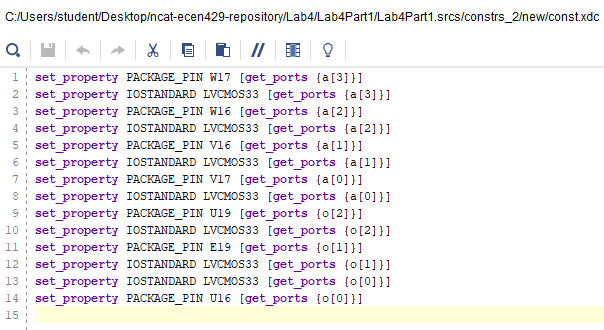
\includegraphics[width=0.5\textwidth]{../report-images/Part1Const.png}
	\caption{\label{fig:Part1ConstFile}Constraints file for Problem 1.}
\end{center}
\end{figure}

\section{Problem 2 VHDL Code}
\begin{lstlisting}[language=VHDL]

\end{lstlisting}

\section{Problem 2 Constraints File}
\begin{figure}[H]
\begin{center}
	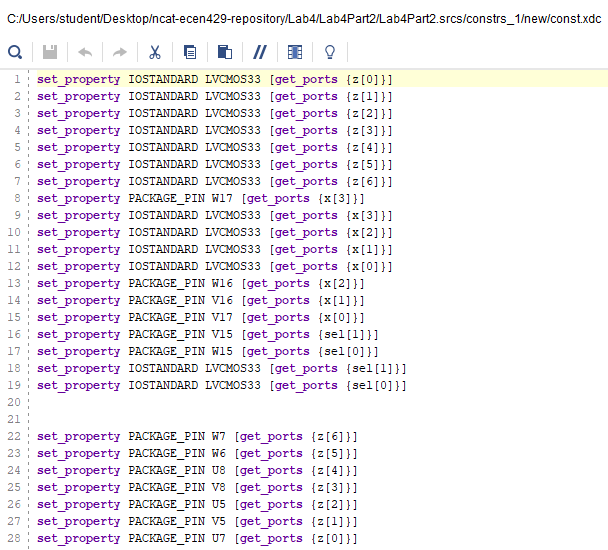
\includegraphics[width=0.5\textwidth]{../report-images/Part2Const.png}
	\caption{\label{fig:Part2ConstFile}Constraints file for Problem 2.}
\end{center}
\end{figure}

\end{appendices}
\end{document}
